\begin{figure}%
    \centering
    \subfloat[]{{\includegraphics[width=7cm]{./figures/CalibratedSpectrum.pdf }}%
    \quad
    \subfloat[]{{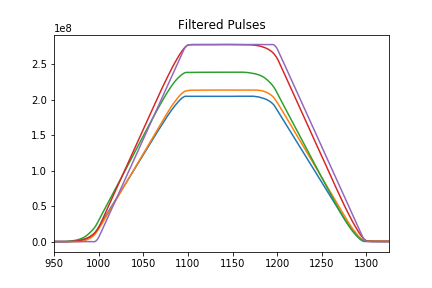
\includegraphics[width=7cm]{./figures/tenevents_filtered.pdf} }}%
    \caption{A CALIBRATED ENERGY SPECRUM}%
    \label{spectrum}%
\end{figure}




Five signals were chosen from the ${}^{137}${Cs} data set. The raw signals are plotted in Figure \ref{fig:signals}, after a baseline correction. The resultant signals after usage of the trapezoidal filter with a gap time and peaking time of 1 $\mu$s are also plotted. The correlation between amplitudes of raw and filtered signals is apparent. Additionally, the effect of signal rise-time can be observed. The signal in purple exhibits the most ideal behavior. This signal has the fastest rise-time and most-closely resembles an ideal step function. All charge is collected quickly; none is lost. The red signal is of the same amplitude but has a longer rise time. As expected, the resultant filtered signal is less ideal, showing more curved corners and more variation in amplitude in the flat top region. These effects, if pronounced, can lead to degraded energy resolution.

Deleterious effects of short gap times were observed. For short gap times, the peak position is shifted down in energy. Also, the peak is broader and tends to have low-energy tailing leading to non-Gaussian peaks. Some of this is likely due to ballistic deficit. A plot of resolution as a function of gap time is shown in Figure \ref{gap}. For gap times greater than a certain amount ($\approx$250 ns), no significant variation in energy resolution with increasing gap time was observed. This value corresponds well to the expected value for the maximum transit time for charge carriers expected in a small ($\approx$ 4.5 cm diameter) coaxial HPGe detector \cite{Knoll} ),

\begin{figure}
\begin{centering}
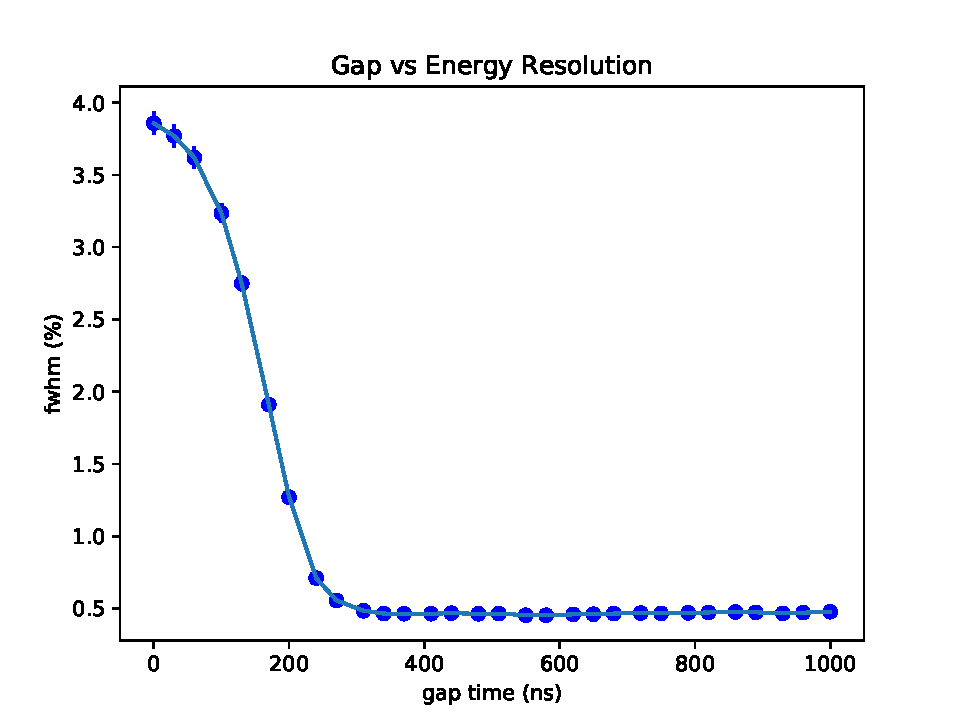
\includegraphics[width=0.7\textwidth]{gap_optimization_cs.pdf}
\caption{Energy resolution as a function of gap time for the 1173 keV peak in ${}^{60}$Co. The peaking time was kept fixed at 500 ns. The minimum FWHM occurs at a gap time of 450 ns. The error bars account for fitting errors and are too small to be seen on most points.}
\label{gap}
\end{centering}
\end{figure}
\begin{figure}
\begin{centering}
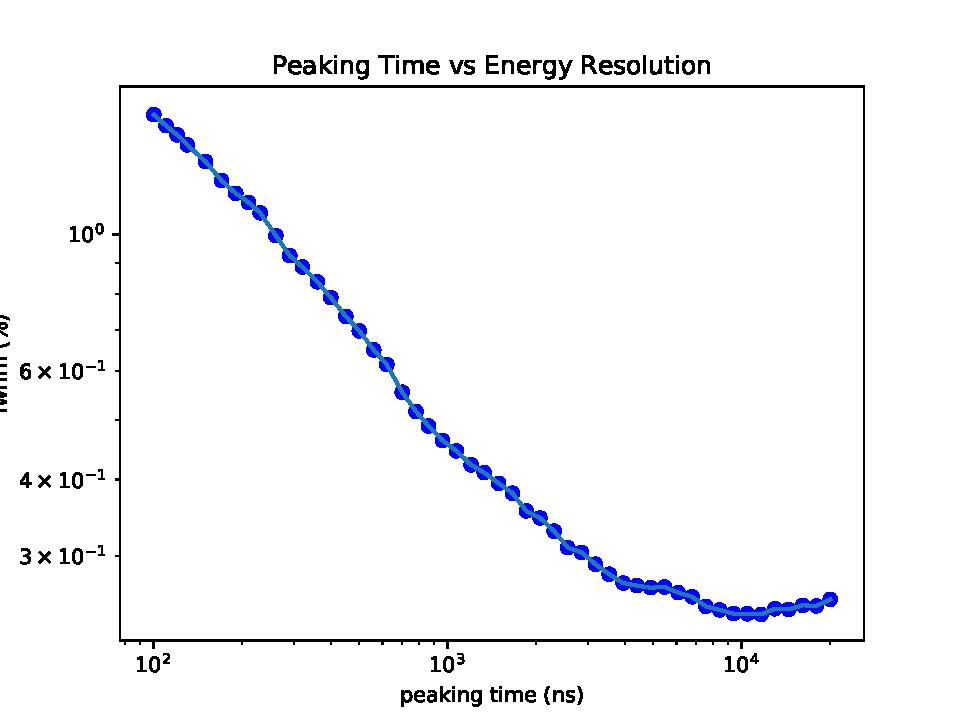
\includegraphics[width=0.7\textwidth]{peak_optimization_cs.pdf}
\caption{Energy resolution as a function of peaking time for the 1173 keV peak in ${}^{60}$Co. The gap time was kept fixed at 450 ns. The minimum fwhm occurs are a peaking time of 10 $\mu$s. The error bars account for fitting errors and are too small to be seen on most points.}
\label{peak}
\end{centering}
\end{figure}

A plot of resolution as a function of peaking time is shown in Figure \ref{peak}. The optimal peaking time is $\approx $ 10 $\mu$s. This is a reasonable optimal peaking time for such a system. From Figure \ref{peak} we can see that our system has relatively low parallel noise (typically dominated by detector leakage current) and high series noise (dominated by capacitance) in the examined range of peaking times.

\begin{figure}
\begin{centering}
\includegraphics[width=0.7\textwidth]{fwhm_vs_energy.pdf}
\caption{Energy resolution as a function of gamma energy is plotted. The error bars account for fitting errors and are too small to be seen on most points.}
\label{eres}
\end{centering}
\end{figure}

The energy resolution as a function of gamma ray energy is plotted in Figure \ref{eres}. The poor energy resolution of the lowest energy is partially due to difficult with fitting the ${}^{241}$Am peak.

Using these values the Fano factor, the ratio of the observed variance in the number of charge carriers to the predicted variance in number for a Poisson process, can be calculated.

\begin{equation}
(FWHM)^{2}_{overall} = (FWHM)^{2}_{statistical}+ (FWHM)^{2}_{electronic} + (FWHM)^{2}_{chargeloss}
\end{equation}
\vspace{5mm}

Assuming that charge loss is negligible in our system,

\vspace{5mm}
\begin{equation}
(FWHM)^{2}_{statistical} = (FWHM)^{2}_{overall} - (FWHM)^{2}_{electronic}
\end{equation}
\begin{equation}
(FWHM)^{2}_{statistical} = 2.35 \times \sqrt{F \epsilon E}
\end{equation}
\vspace{5mm}

where $F$ is the Fano factor, $E$ is the energy of the gamma-ray, and $\epsilon$ is the average energy needed to create an 
electron hole pair (2.9 eV /cit{knoll}). Thus,

\vspace{5mm}
\begin{equation}
F = ((FWHM)^{2}_{overall} - (FWHM)^{2}_{electronic}) \frac{1}{2.35 \epsilon E}
\end{equation}
\vspace{5mm}

A Fano factor was calculated for each of four energy peaks.
  
A pulser input was used in each data set. The pulser peak is meant to provide a measure of electronic noise since the resolution of the pulser peak is decoupled from charge loss, carrier statistics, and other detector-dependent noise sources. There was some variation in the pulser peak resolution with energy, likely due to background and imperfect fitting. The average pulser resolution was used in calculating the Fano factor. Of the four calculated values, the one corresponding to the ${}^{241}$Am peak was very different than the other values. This is likely because the background for this peak is the most considerable and leads to errors in peak fitting with a simple linear background. This value was discarded. An average of the other three fano factor values gives $F = 0.035 \pm0.017$.

The calculated Fano factor is significantly different from the approximate value of $\approx 0.12$ \cite{Knoll}. Using different filter parameters (optimized with the 1132 keV peak of ${}^{60}$Co) of a gap time of 450 ns and a rise time of 15$\mu$s, the fano factor was found to be$ 0.094 \pm 0.026$. Initially the ${}^{60}$Co parameters were discarded (due to larger fitting errors) in favor of the $^{137}$Cs parameters. The large change in Fano factor value indicates that perhaps the filter is not optimized as well as it could be for best treatment of all of energy peaks. Optimizing the filter separately for each peak would probably give better performance and less error.